\section{Theorie} \label{sec:Theorie}

\subsection{Grundprinzip der elektrischen Brückenschaltungen}

   Elektrische Brückenschaltungen werden dazu verwendet, um unbekannte Größen, wie zum Bespiel Widerstände, Induktivitäten und
   Kapazitäten zu bestimmen.
   Dazu wird die Potentialdifferenz $U_\text{Br}$ zwischen zwei Punkten an der Schaltung gemessen.
   Mithilfe der Kirchhoff'schen Regeln lässt sich diese Brückenspannung $U_\text{Br}$ berechnen.
   \begin{enumerate}
       \item Die Knotenregel besagt, dass alle Ströme, die in einen Knoten hineinfließen, in der Summe gleich Null sein müssen.
       \begin{equation}
           \sum_k I_k = 0
       \end{equation}
       \item Die Maschenregel besagt, dass in einer Masche alle vorhandenen Spannungen in der Summe gleich Null sein müssen.
       \begin{equation}
           \sum_k U_k = 0
       \end{equation}
   \end{enumerate}

   % IMPROVE: Grafik zur allgemeinen Brückenschaltung
   % \includegraphics[scale=0.8]{content/img/allg-bruecke.svgz}
   % \input{content/tikz/bruecke-maxwell.tex}

   Daraus folgt für die allgemeine Brückenspannung:

   \begin{equation}
       U_\text{Br} = \frac{R_2R_3 - R_1R_4}{(R_3 + R_4)(R_1 + R_2)} U_\text{S}
   \end{equation}
   Hierbei ist $U_\text{S}$ die Speisespannung des Stromkreises.
   Für das Verhältnis
   \begin{equation}
       R_1R_4 = R_2R_3 \label{eqn:Widerstände}
   \end{equation}
   verschwindet die Brückenspannung und man spricht von einer abgeglichenen Brücke.
   In den Brückenschaltungen sind Bauelemente enthalten, die als Abgleichelemente dienen.
   Dies sind Potentiometer, mit denen sich die ohmschen Widerstände in den Schaltungen variieren lassen, um
   die Brückenspannung auf Null zu regeln.
   Da die Speisespannung proportional zur Brückenspannung ist, sollte die Speisespannung möglichst hoch eingestellt werden,
   damit eine höhere Abgleichempfindlichkeit erzielt wird.
   Ziel ist es also, um eine unbekannte Größe zu bestimmen, die gegebenen Bauteile so einzustellen, dass
   die Brückenspannung gleich Null wird. Dann kann man aus den Beziehungen der bekannten Größen die Größen für das unbekannte Bauteil berechnen.

\subsection{Bestimmung der unbekannten Größen}

    \subsubsection{Messung von ohmschen Widerständen} \label{sec:Wheatstone}

        \usetikzlibrary{circuits.ee.IEC}

\tikzset{circuit declare symbol = AC source}
\tikzset{AC source IEC graphic/.style={
    circuit symbol lines,
    circuit symbol size=width 2 height 2,
    shape=generic circle IEC,
    /pgf/generic circle IEC/before background={
    \pgfpathmoveto{\pgfpoint{-0.8pt}{0pt}}
    \pgfpathsine{\pgfpoint{0.4pt}{0.4pt}}
    \pgfpathcosine{\pgfpoint{0.4pt}{-0.4pt}}
    \pgfpathsine{\pgfpoint{0.4pt}{-0.4pt}}
    \pgfpathcosine{\pgfpoint{0.4pt}{0.4pt}}
    \pgfusepath{stroke}
    },
    transform shape, draw
  }
}
\tikzset{circuit ee IEC/.append style=
  {set AC source graphic = AC source IEC graphic}
}

\begin{figure}
    \centering
    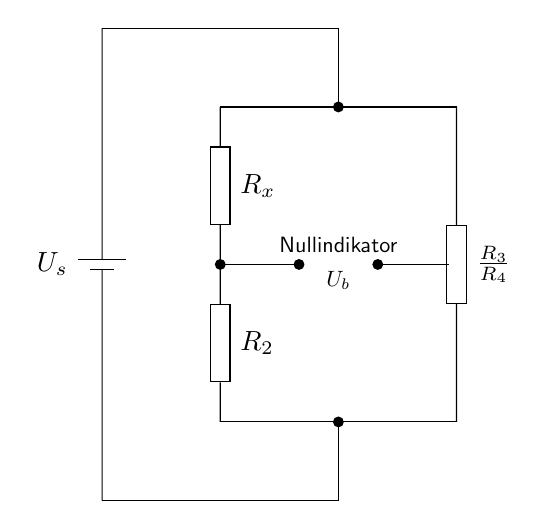
\begin{tikzpicture}[circuit ee IEC, font=\sffamily]
    \draw (0,0) to [battery={info'={$U_s$}}] (0,-6);
    \draw (0,0) -- (3,0);
    \draw (3,0) -- (3, -1);
    \node[contact] at (3,-1) {};
    \draw (1.5, -1) -- (4.5, -1);
    \draw (1.5, -1) to [resistor={info={$R_x$}}] (1.5, -3);
    \draw (1.5, -3) to [resistor={info={$R_2$}}] (1.5, -5);

    % \draw (4.5, -1) to [resistor={info={$R_3$ \\ $R_4$}}] (4.5, -5);
    % \draw (4.5, -1) to [resistor={info={$R_3$ / $R_4$}}] (4.5, -5);
    \draw (4.5, -1) to [resistor={info={$\frac{R_3}{R_4}$}}] (4.5, -5);

    \node[scale=0.8] at (3,-2.75) {Nullindikator};
    \node[scale=0.8] at (3,-3.2) {$U_b$};
    \node[contact] at (1.5,-3) {};
    \node[contact] at (2.5, -3) {};
    \node[contact] at (3.5,-3) {};
    \draw (1.5, -3) -- (2.5, -3);
    \draw (3.5, -3) -- (4.4, -3);
    \draw (1.5, -5) -- (4.5, -5);
    \node[contact] at (3,-5) {};
    \draw (0, -6) -- (3,-6);
    \draw (3, -6) -- (3,-5);
    \end{tikzpicture}
    \caption{Wheatstone-Brücke}
    % \label{fig:Wheatstone Brücke}
\end{figure}


        Um unbekannte Widerstände zu bestimmen, wird die Wheatstone'sche Brückenschaltung verwendet.
        Diese besteht nur aus ohmschen Widerständen und kann mit Gleich- und Wechselstrom betrieben werden.
        Der unbekannte Widerstand kann mithilfe der Gleichung \eqref{eqn:Widerstände} berechnet werden.
        Es gilt
        \begin{equation}
            R_x = R_2 \frac{R_3}{R_4} \; . \label{eqn:Rx}
        \end{equation}
        Die schon bekannten Widerstände sind $R_2$, $R_3$ und $R_4$. \,
        $\frac{R_3}{R_4}$ kann durch ein Potentiometer so eingestellt werden,
        dass die Brückenspannung $U_\text{Br}$ gleich Null wird.
        Mit den so eingestellten Widerständen können die Größen für das unbekannte Bauteil berechnet werden.

    \subsubsection{Komplexe Widerstände}

        Bei der Verwendung von Kondensatoren mit einer Kapazität $C$ und Spulen mit einer Induktivität $L$ werden bei der Berechnung
        komplexe Widerstände verwendet. Als Speisespannung wird eine Wechselspannung eingesetzt.
        Komplexe Widerstände setzen sich aus einem Wirkwiderstand $X$ und einem Blindwiderstand $Y$ zusammen.
        Die allgemeine Darstellung lautet
        \begin{equation}
            \symbf{R} = X + jY \; .
        \end{equation}
        Für ohmsche Widerstände $R$, Kapazitäten $C$ und Induktivitäten $L$ werden durch
        \begin{align}
            \symbf{R}_R = R \,, && \symbf{R}_C = - \frac{j}{\omega C} \,, && \symbf{R}_L = j \omega L
        \end{align}
        dargestellt.

    \subsubsection{Messung von Kapazitäten} \label{sec:Kapazität}

        % \usetikzlibrary{circuits.ee.IEC}

\tikzset{circuit declare symbol = AC source}
\tikzset{AC source IEC graphic/.style={
    circuit symbol lines,
    circuit symbol size=width 2 height 2,
    shape=generic circle IEC,
    /pgf/generic circle IEC/before background={
    \pgfpathmoveto{\pgfpoint{-0.8pt}{0pt}}
    \pgfpathsine{\pgfpoint{0.4pt}{0.4pt}}
    \pgfpathcosine{\pgfpoint{0.4pt}{-0.4pt}}
    \pgfpathsine{\pgfpoint{0.4pt}{-0.4pt}}
    \pgfpathcosine{\pgfpoint{0.4pt}{0.4pt}}
    \pgfusepath{stroke}
    },
    transform shape, draw
  }
}
\tikzset{circuit ee IEC/.append style=
  {set AC source graphic = AC source IEC graphic}
}

\begin{figure}
    \centering
    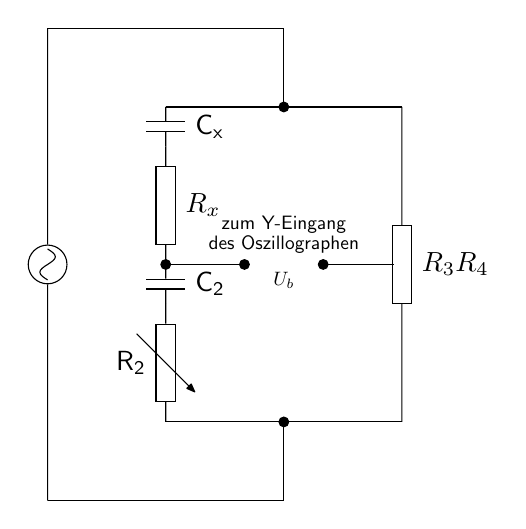
\begin{tikzpicture}[circuit ee IEC, font=\sffamily]
    \draw (0,0) to [AC source](0,-6);
    \draw (0,0) -- (3,0);
    \draw (3,0) -- (3, -1);
    \node[contact] at (3,-1) {};
    \draw (1.5, -1) -- (4.5, -1);
    \draw (1.5,-1) to [capacitor={info={C$\mathsf{_{x}}$},info'={$\mathsf{_{}}$}}] (1.5,-1.5);
    \draw (1.5, -1.5) to [resistor={info={$R_x$}}] (1.5, -3);
    \draw (1.5,-3) to [capacitor={info={C$\mathsf{_{2}}$},info'={$\mathsf{_{}}$}}] (1.5,-3.5);
    \draw (1.5, -3.5) to  [resistor={adjustable={info={$\mathsf{_{}}$}}, info'={R$\mathsf{_{2}}$}}] (1.5,-5);
    \draw (4.5, -1) to [resistor={info={$R_3$ \\ $R_4$}}] (4.5, -5);
    \node[scale=0.7] at (3, -2.5) {zum Y-Eingang};
    \node[scale=0.7] at (3,-2.75) {des Oszillographen};
    \node[scale=0.7] at (3,-3.2) {$U_b$};
    \node[contact] at (1.5,-3) {};
    \node[contact] at (2.5, -3) {};
    \node[contact] at (3.5,-3) {};
    \draw (1.5, -3) -- (2.5, -3);
    \draw (3.5, -3) -- (4.4, -3);
    \draw (1.5, -5) -- (4.5, -5);
    \node[contact] at (3,-5) {};
    \draw (0, -6) -- (3,-6);
    \draw (3, -6) -- (3,-5);
    \end{tikzpicture}
    \caption{Kapazitätsmessbrücke}
    % \label{fig:Kapazitätsmessbrücke}
\end{figure}


        Da bei einem realen Kondensator immer ein Teil der elektrischen Energie in Wärmeenergie umgewandelt
        wird und so verloren geht, wird mit dem Kondensator ein ohmscher Widerstand in Reihe geschaltet.
        Dieser ohmsche Widerstand wird mit Gleichung \eqref{eqn:Rx} berechnet.
        Für die Kapazität des Kondensators gilt
        \begin{equation}
            C_x = C_2 \frac{R_4}{R_3} \; . \label{eqn:Cx}
        \end{equation}
        Die Kapazität $C_2$ ist hierbei schon bekannt und ist mit einem Potentiometer, welches den bekannten Widerstand $R_2$ regelt,
        in Reihe geschaltet.

    \subsubsection{Messung von Induktivitäten} \label{sec:Induktivität}

        % IMPROVE: Datei identisch zur Maxwell-Brücke…
        % \input{content/tikz/induktivitaetsmessbruecke.tex}

        Auch bei einer realen Induktivität wird ein Teil der enthaltenen magnetischen Feldenergie in Wärmeenergie umgewandelt
        und geht verloren. Aus diesem Grund wird auch hier ein ohmscher Widerstand mit der Induktivität, zum Beispiel einer Spule,
        in Reihe geschaltet.
        Der ohmsche Widerstand kann wieder mit Gleichung \eqref{eqn:Rx} bestimmt werden.
        Die Induktivität wird durch
        \begin{equation}
            L_x = L_2 \frac{R_3}{R_4} \label{eqn:Lx}
        \end{equation}
        berechnet.
        Die Induktivität $L_2$ ist hier ebenfalls schon bekannt, und mit dem Potentiometer für $R_2$ in Reihe geschaltet.

    \subsubsection{Maxwell-Brücke} \label{sec:Maxwell}

        \usetikzlibrary{circuits.ee.IEC}

\tikzset{circuit declare symbol = AC source}
\tikzset{AC source IEC graphic/.style={
    circuit symbol lines,
    circuit symbol size=width 2 height 2,
    shape=generic circle IEC,
    /pgf/generic circle IEC/before background={
    \pgfpathmoveto{\pgfpoint{-0.8pt}{0pt}}
    \pgfpathsine{\pgfpoint{0.4pt}{0.4pt}}
    \pgfpathcosine{\pgfpoint{0.4pt}{-0.4pt}}
    \pgfpathsine{\pgfpoint{0.4pt}{-0.4pt}}
    \pgfpathcosine{\pgfpoint{0.4pt}{0.4pt}}
    \pgfusepath{stroke}
    },
    transform shape, draw
  }
}
\tikzset{circuit ee IEC/.append style=
  {set AC source graphic = AC source IEC graphic}
}

\begin{figure}
   \centering
   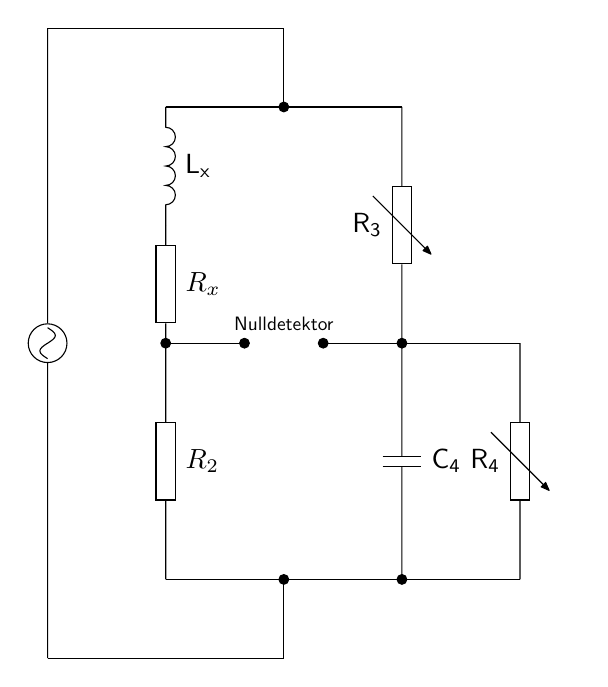
\begin{tikzpicture}[circuit ee IEC, font=\sffamily]
   \draw (0,0) to [AC source](0,-8);
   \draw (0,0) -- (3,0);
   \draw (3,0) -- (3, -1);
   \node[contact] at (3,-1) {};
   \draw (1.5, -1) -- (4.5, -1);
   \draw (1.5,-1) to [inductor={info={L$\mathsf{_{x}}$},info'={$\mathsf{_{}}$}}] (1.5,-2.5);
   \draw (1.5, -2.5) to [resistor={info={$R_x$}}] (1.5, -4);
   \draw (1.5, -4) to [resistor={info={$R_2$}}] (1.5, -7);
   \draw (4.5, -1) to  [resistor={adjustable={info={$\mathsf{_{}}$}}, info'={R$\mathsf{_{3}}$}}] (4.5,-4);
   \node[scale=0.7] at (3,-3.75) {Nulldetektor};
   \node[contact] at (1.5,-4) {};
   \node[contact] at (2.5, -4) {};
   \node[contact] at (3.5, -4) {};
   \node[contact] at (4.5, -4) {};
   \draw (1.5, -4) -- (2.5, -4);
   \draw (3.5, -4) -- (4.5, -4);
   \draw (1.5, -7) -- (4.5, -7);
   \node[contact] at (3,-7) {};
   \draw (4.5,-4) to [capacitor={info={C$\mathsf{_{4}}$},info'={$\mathsf{_{}}$}}] (4.5,-7);
   \node[contact] at (4.5, -7) {};
   \draw (6, -4) to  [resistor={adjustable={info={$\mathsf{_{}}$}}, info'={R$\mathsf{_{4}}$}}] (6,-7);
   \draw (4.5, -7) -- (6,-7);
   \draw (4.5, -4) -- (6,-4);
   \draw (0, -8) -- (3,-8);
   \draw (3, -8) -- (3,-7);
   \end{tikzpicture}
   \caption{Induktivitätsmessbrücke}
   % \label{fig:Induktivitätsmessbrücke}
\end{figure}


        Eine weitere Möglichkeit, um Induktivitäten zu bestimmen, ist die Maxwell'sche Brückenschaltung.
        Die Elemente zum Abgleichen der Brücke sind hier $R_2$, $R_3$, $R_4$ und $C_4$, wobei $R_3$ und $R_4$ durch ein
        Potentiometer geregelt werden. Die Kapazität $C_4$ ersetzt die Induktivität $L_2$, da dies
        einfacher zu realisieren ist.
        Der Widerstand, der mit der Induktivität in Reihe geschaltet ist, lässt sich durch Gleichung \eqref{eqn:Rx} bestimmen,
        die Induktivität wird mit
        \begin{equation}
            L_x = R_2 R_3 C_4 \label{sec:LxMax}
        \end{equation}
        berechnet.

\subsection{Frequenzabhängige Brückenschaltungen}

    Alle komplexen Widerstände sind von der Frequenz $\omega$ der Speisespannung $U_\text{S}$ abhängig.
    Ist diese Frequenz zu hoch eingestellt, wird der Anteil der Streukapazitäten, die in den Bauteilen
    entstehen, zu groß, und ein Abgleichen ist nicht mehr möglich.
    Wenn die Frequenz zu niedrig ist, kommt es zu Problemen bei der technischen Handhabung,
    da nun einige Periodendauern für Einschwingvorgänge benötigt werden, bis sich eine stabile Brückenspannung $U_\text{Br}$
    eingestellt hat.
    Die Frequenzen sind optimal, wenn sich die Blind- und Wirkwiderstände einer Schaltung
    in einer Größenordnung befinden.

    \subsubsection{Die Wien-Robinson-Brücke} \label{sec:WR}

        In der Schaltung der Wien-Robinson-Brücke sind keine Abgleichelemente enthalten.
        Die Brückenspannung $U_\text{Br}$ soll in Abhängigkeit der Frequenz $\omega$ bestimmt werden.
        Es gilt:
        \begin{equation}
        \label{eqn:WienRobinsonBrNachS}
            \left\lvert \frac{U_\text{Br}}{U_\text{S}} \right\rvert^2
            = \frac{1}{9} \frac{(\Omega^2 - 1)^2}{(1 - \Omega^2)^2 + 9\Omega^2}
            \; ,
        \end{equation}
        wobei
        \begin{equation}
            \Omega = \frac{\omega}{\omega_0} \label{eqn:GroßOmega}
        \end{equation}
        ist, mit
        \begin{equation}
            \omega_0 = \frac{1}{RC} \; . \label{eqn:omeganull}
        \end{equation}

        Die Wien-Robinson-Brücke filtert aus dem kontinuierlichen Frequenzspektrum die Frequenz $\omega_0$ heraus
        und schwächt die Frequenzen in der Nähe von $\omega_0$.
        Mit dieser Eigenschaft soll der Klirrfaktor gemessen werden, welcher dazu dient, die Qualität des
        Sinusgenerators zu prüfen.
        Wenn der Klirrfaktor hinreichend klein ist, ist auch der Anteil der Oberwellen, welche bei einem
        realen Sinusgenerator entstehen, gering.
        Der Generator wird auf die Frequenz $\omega_0$ geregelt, und übrig bleiben nur die von $\omega_0$
        verschiedenen Frequenzen.

    \subsubsection{Die TT-Brücke}

        Die TT-Brücke dient wie die Wien-Robinson-Brücke als elektronischer Filter.
        Der Unterschied liegt darin, dass die Spannungen $U_\text{S}$ und $U_\text{Br}$ gegen Masse
        angeschlossen werden können.
        Für das Spannungsverhältnis ergibt sich mit den Bezeichnungen
        aus den Gleichungen \eqref{eqn:GroßOmega} und \eqref{eqn:omeganull}:
        \begin{equation}
            \left\lvert \frac{U_\text{Br}}{U_\text{S}} \right\rvert = \frac{(\Omega^2 - 1)^2}{(1 - \Omega^2)^2 + 16\Omega^2}.
        \end{equation}
